\section{Sicherheitsarchitektur iOS}
	\subsection{Secure boot chain}
	Apple hat eine Kette aneinander gereihter, vom Vorg�nger abh�ngiger Prozesse
	entwickelt, um den Startvorgang m�glichst abzusichern und eine Manipulation
	der Low-Level Software auszuschlie�en, da iOS nur auf Ger�ten startet, welche
	auf diesem Wege erfolgreich validiert wurden. Dieses "`secure boot chain"'
	genannte Verfahren sieht vor, nach dem Start eines iOS Ger�tes zuerst
	Code aus einem nur lesbaren Speicherbereich auszuf�hren. Dieser hardware of
	trust genannte unver�nderbare Code ist bei der Manufaktur der Chips eingebettet 
	worden und somit implizit vertraulich. Das Boot ROM enth�lt zus�tzlich Apple's 
	�ffentlichen Schl�ssel des Root Zertifikats, welcher sicher stellt, dass der 
	Low-Level-Bootloader von Apple signiert ist, bevor er ausgef�hrt wird. 
	
	%\begin{figure}[h]
		%\centering
 		%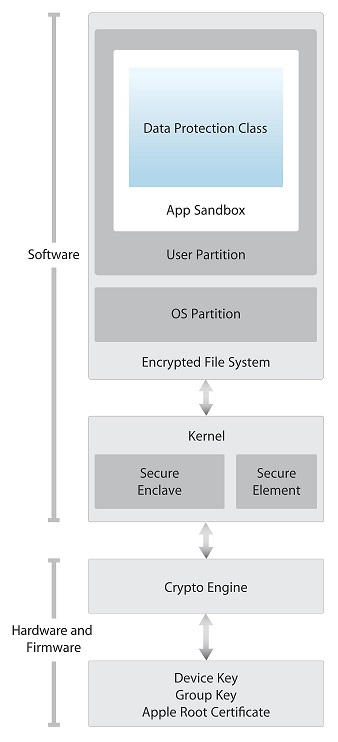
\includegraphics[width=0.3\linewidth]{ios/media/security-model.jpg}
        %\caption{Sicherheitsarchitektur Diagramm von iOS}
        %\label{fig:security-model}
    %\end{figure}\\
    %ref: Figure \ref{fig:security-model} shows the sec. arch.
    
    %\begin{wrapfigure}[Zeilen]{Position}[Ueberhang]{Breite}
	\begin{wrapfigure}[0]{r}[0.5cm]{6cm}
		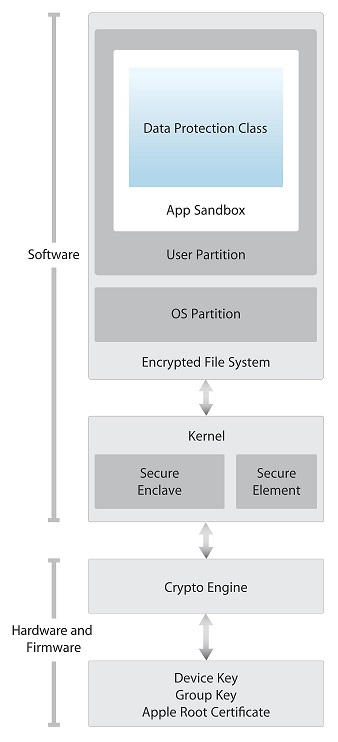
\includegraphics[width=\linewidth]{ios/media/security-model.jpg}
		\caption{Sicherheitsmodel von iOS}
		\label{fig:security-model}
	\end{wrapfigure}
	\subsection{iOS Sicherheitsmodel}
	Apple integrierte vier Schichten der Sicherheit in iOS.\\